\documentclass[dvipdfmx]{beamer} %通常用
%\documentclass[dvipdfm,handout]{beamer} #ハンドアウト作成用

\AtBeginDvi{\special{pdf:tounicode 90ms-RKSJ-UCS2}} % 栞の文字化けを制御(日本語の場合必須)
\setbeamertemplate{navigation symbols}{} %ナビゲーションバーを消す

\usepackage{comment}
\usepackage{amsmath}
\usepackage{algorithm}
\usepackage{algorithmic}

%%% 以下2つはハンドアウト印刷用
%\usepackage{pgfpages}
%\pgfpagesuselayout{4 on 1}[border shrink=3mm]

%%% 付録をページ番号に含めないためのコマンド
\newcommand{\backupbegin}{
\newcounter{framenumberappendix}
\setcounter{framenumberappendix}{\value{framenumber}}
}
\newcommand{\backupend}{
\addtocounter{framenumberappendix}{-\value{framenumber}}
\addtocounter{framenumber}{\value{framenumberappendix}}
}

%%% メインテーマ
%\usetheme{Berkeley}
%\usetheme{CambridgeUS}
%\usetheme{Default}
%\usetheme{Darmstadt}
%\usetheme{Hannover}
%\usetheme{lankton-keynote}
%\usetheme{Luebeck}
%\usetheme{Marburg}
\usetheme{Madrid}
%\usetheme{boxes}
%\usetheme{Bergen}
%\usetheme{Boadilla}
%\usetheme{Pittsburgh}
%\usetheme{Rochester}

%%% テーマ
%\useinnertheme{rectangles}
%\useoutertheme{default}

%%% カラーテーマ(省略可)
%\useoutertheme{infolines}
%\usecolortheme[RGB={64,64,64}]{structure}     
%\definecolor{babyblue}{rgb}{0.54,0.81,0.94}                                                                                                
%\usecolortheme{dolphin}
%\usecolortheme{beaver}
%\usecolortheme{beetle}
%\usecolortheme{crane}
%\usecolortheme{dolphin}
%\usecolortheme{seagull}
%\usecolortheme{wolverine}
%\usecolortheme{spruce}
%\usecolortheme{rose}
%\usecolortheme{seahorse}
\setbeamertemplate{footline}[page number]

%%% フォント
\renewcommand{\kanjifamilydefault}{\gtdefault} % 日本語フォントをゴシック
\usefonttheme[onlymath]{serif}
\usefonttheme[onlylarge]{structurebold}
%\usefonttheme{professionalfonts}
\fontencoding{\encodingdefault}
\fontfamily{\kanjifamilydefault}
\fontseries{\seriesdefault}
\fontshape{\shapedefault}
\selectfont
%\mathversion{bold} % 数式フォントをbold体

%%% インナー, アウターテーマ(省略可)
%\useinnertheme{circles}
%\useoutertheme{infolines}

%\logo{\includegraphics[width=1.5cm, height=1.5cm]{.jpg}} % ロゴをいれる
\setbeamertemplate{navigation symbols}{} % ナビゲーションバーなし
%\setbeamertemplate{background}[grid][step=5mm] % 背景グリッド
\setbeamertemplate{footline}[frame number] % ページ番号の表示
\setbeamerfont{footline}{size=\small,series=\bfseries}
\setbeamercolor{footline}{fg=black,bg=black}
\setbeamertemplate{caption}[numbered] % 図表番号の表示
%\setbeamerfont*{frametitle}{size=\normalsize,series=\bfseries} % フレーム文字の大きさ
\setbeamerfont*{frametitle}{size=\large,series=\bfseries} % フレームごとのフォントを設定変更できる。
\setbeamertemplate{frametitle}[default][center] % タイトルを中央寄せに設定変更できる。

\definecolor {mycolor1} {rgb} {0.00, 0.39, 0.00}
\definecolor {mycolor2} {rgb} {0.55, 0.27, 0.07}
\definecolor {mycolor3} {rgb} {0.63, 0.13, 0.94}

\definecolor {mycolorTitle} {rgb} {0.85, 0.855, 0.85}
\definecolor {mycolorHeader} {rgb} {0.93, 0.935, 0.93}

%ヘッダーとタイトルの色(fgで文字の色変えられる)
%\setbeamercolor{frametitle}{bg = mycolorHeader}
%\setbeamercolor{title}{bg = mycolorTitle}

\def\conpage{7}

%%% パッケージ
\usepackage[japanese]{babel}
\usepackage{inputenc}
\usepackage{times}
\usepackage{amsmath}
\usepackage{amssymb}
\usepackage{amsfonts}
\usepackage[T1]{fontenc}
\usepackage{hyperref}
\usepackage{algorithm,algorithmic}
\usepackage{ascmac}
%\usepackage{txfonts}
\usepackage{color}
%\usepackage{algpseudocode,algorithm}
%\usepackage{tikz}
%\usetikzlibrary{arrows}
%\tikzstyle{block}=[fill=blue,draw opacity=0.7,line width=1.4cm]

%\makeatletter
%\renewcommand{\thealgorithm}{%
%\thesection.\arabic{algorithm}}
%\@addtoreset{algorithm}{section}
%\makeatother

%\usepackage{listings,jlisting}
\usepackage{listings}

\lstset{%
  language={R},
  basicstyle={\small},%
  identifierstyle={\small},%
  commentstyle={\small\itshape},%
  keywordstyle={\small\bfseries},%
  ndkeywordstyle={\small},%
  stringstyle={\small\ttfamily},
  frame={tb},
  breaklines=true,
  columns=[l]{fullflexible},%
  numbers=left,%
  xrightmargin=0zw,%
  xleftmargin=3zw,%
  numberstyle={\scriptsize},%
  stepnumber=1,
  numbersep=1zw,%
  lineskip=-0.5ex%
}

\newcommand{\bm}[1]{\mbox{\boldmath $#1$}}
\newcommand{\mapright}[1]{\mathop{\longrightarrow}\limits_{#1}}
\newcommand{\argmax}{\mathop{\rm argmax}\limits}

\renewcommand{\figurename}{図}
\renewcommand{\tablename}{表}

%%% Title, Author, etc.
\title[タイトル]{混合射影正規分布によるクラスタリングについて}
%\subtitle[サブタイトル]{}
\author[発表者名]{塩濱研究室\\ 小坪琢人}
\institute[所属]{東京理科大学\ 工学部経営工学科4年\\学籍番号 4414036}
\date[日付]{2018年1月30日}

\begin{document}

\begin{frame}[plain]
\titlepage
\end{frame}

\begin{frame}{目次}
\tableofcontents
\end{frame}

%%%%%%%%%%%%% はじめに %%%%%%%%%%%%%%%
\section{はじめに}
\begin{frame}{はじめに}

\begin{itemize}

\item 
円周上や球面上のデータを扱う統計手法を方向統計学といい, 近年多様体上の統計分析
手法として, 注目を集めている.

\item 
単位超球面上$(\mathbb{S}^{p-1})$ に分布するようなデータをユークリッド空間上のデータとして扱い, ベクトル間の類似度の指標にユークリッド距離を用いると良い解析が行えない場合がある.

\end{itemize}

\begin{figure}[H]
 \begin{tabular}{c}
 %\hspace{0.5cm}
 \begin{minipage}{0.5\hsize}
  \begin{center}
   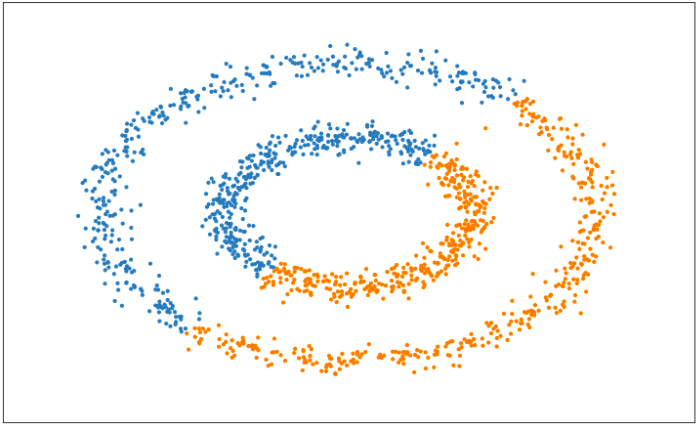
\includegraphics[clip,height= 30mm]{data/sample_mixture_miss2.png}
  \end{center}
 \end{minipage}
 \begin{minipage}{0.5\hsize}
  \begin{center}
 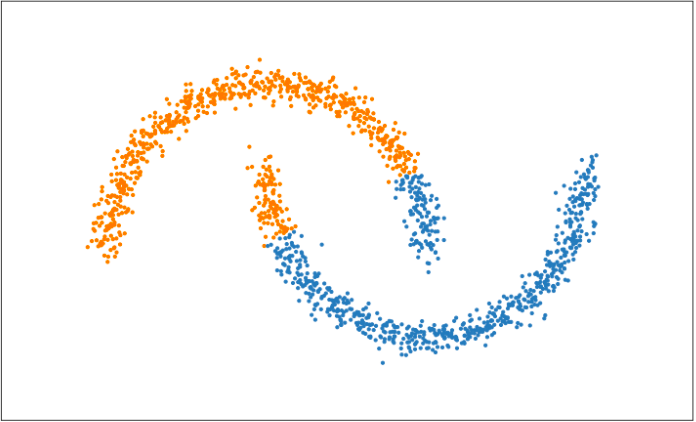
\includegraphics[clip,height= 30mm]{data/sample_mixture_miss1.png}
  \end{center}
 \end{minipage}
\end{tabular}
\caption{混合正規分布による誤った分類結果}
\end{figure}

\end{frame}

\begin{frame}{背景}

\begin{itemize}

\item 
Dhillon and Modha (2001) は, ユークリッド距離に基づく非類似度の尺度を単位球面上に
射影したコサイン非類似度の最小化に基づく超球面上の$k$平均法を提案した.

\item  
超球面上の$k$平均法は確率モデルを仮定しないノンパラメトリックな手法であるのに対
し, パラメトリックな超球面上のクラスタリング手法として, Gopal and Yang (2014) によ
るvon Mises Fisher 分布の混合分布を用いた手法がある.

\end{itemize}

\end{frame}

%%%%%%%%%%%%% 目的 %%%%%%%%%%%%%%%
\section{目的}
\begin{frame}{目的}
\begin{block}{目的}
\begin{itemize}

\item
方向データの分布として知られる, 射影正規分布の混合分布によるクラスタリングの性能評価を行う.

\end{itemize}
\end{block}
\end{frame}

%%%%%%%%%%%%% 混合射影正規分布 %%%%%%%%%%%%%%%
\section{混合射影正規分布}
\begin{frame}{円周上の射影正規分布(1/2)}

Wang and Gelfand (2013)によると, $\mathcal{PN}_2(\bm \mu,\Sigma$)の場合, 単位円上の方向を表す$U = (\cos\Theta, \sin\Theta)^T$における$\theta$の確率密度を以下に示す.

%\vspace{-0.5cm}
\footnotesize
\begin{eqnarray*}
\label{PNC}
p(\theta; \bm \mu, \Sigma) = \frac{1}{2\pi A(\theta)}|\Sigma|^{-\frac{1}{2}}
\exp(C)\left\{1 + \frac{B(\theta)}{\sqrt{A(\theta)}} \frac{\Phi \left(\frac{B(\theta)}{\sqrt{A(\theta)}}\right)}{\phi \left(\frac{B(\theta)}{\sqrt{A(\theta)}}\right)}\right\} I_{[0,2\pi)}(\theta),
\end{eqnarray*}
\normalsize

\noindent
ここで, $\bm u^T = (\cos\theta,\sin\theta), \ A(\theta) = \bm u^T\Sigma^{-1}\bm u, \ B(\theta) = \bm u^T \Sigma^{-1} \bm \mu,$
$\ C = -\frac{1}{2} \bm \mu^T \Sigma^{-1} \bm \mu$であり, $I_{[0,2\pi)} (\cdot)$は指示関数, $\Phi(\cdot), \phi(\cdot)$ は標準正規分布の確率密度関数と累積密度関数である.

\begin{figure}[H]
 \begin{tabular}{c}
 %\hspace{0.5cm}
 \begin{minipage}{0.5\hsize}
  \begin{center}
   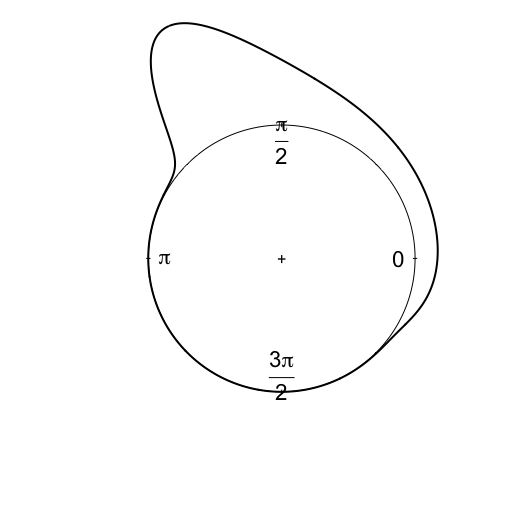
\includegraphics[clip,height= 30mm]{data/sample_asymmetry.png}
  \end{center}
 \end{minipage}
 \hspace{-2.0cm}
 \begin{minipage}{0.5\hsize}
  \begin{center}
 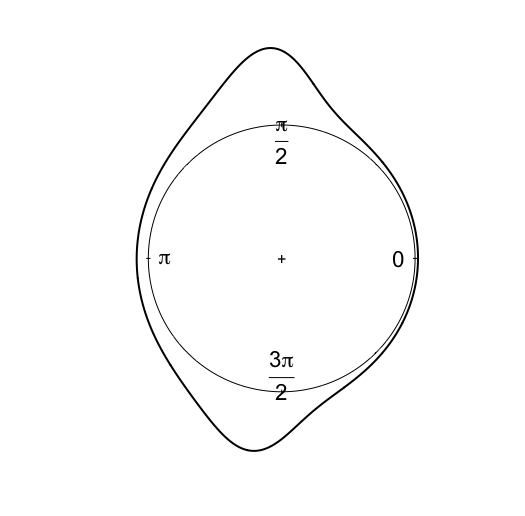
\includegraphics[clip,height= 30mm]{data/sample_bimodal.png}
  \end{center}
 \end{minipage}
\end{tabular}
\caption{射影正規分布の分布例}
\end{figure}

\end{frame}

\begin{frame}{円周上の射影正規分布(2/2)}
% 定義で囲むか, 箱で囲む
\begin{itembox}[l]{平均方向の定義}
二つの角度$\theta_1, \theta_2$(実線)の平均方向は,
\begin{itemize}
	\item
	算術平均では, $\frac{1}{2} (\theta_1 + \theta_2)$(破線)と定義する.
	
	\item 
	円周上では, $\frac{1}{2} (\cos \theta_1 + \cos \theta_2,\sin \theta_1 + \sin \theta_2)$(破線)と定義する.
\end{itemize}
\end{itembox}

\vspace{-0.3cm}
\begin{figure}[H]
 \begin{tabular}{c}
 \begin{minipage}{0.5\hsize}
  \begin{center}
   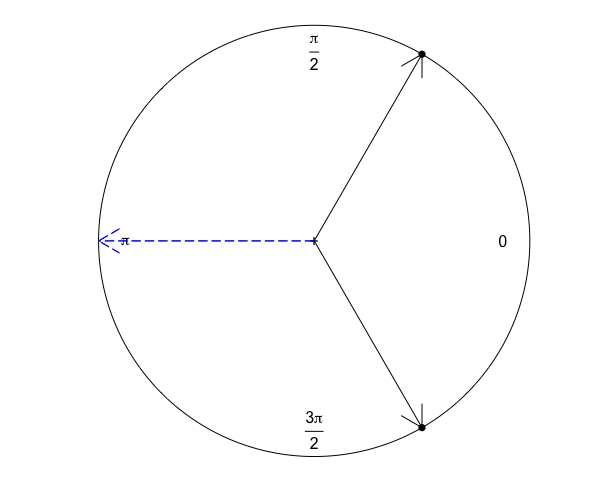
\includegraphics[clip,height= 40mm]{data/sample_False.png}
\caption{算術平均による平均の定義}
\label{sample_mu1}
  \end{center}
 \end{minipage}
 \hspace{-0.5cm}
 \begin{minipage}{0.5\hsize}
  \begin{center}
 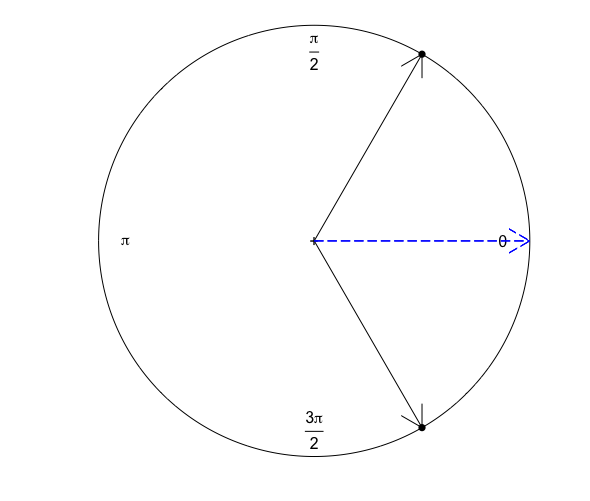
\includegraphics[clip,height= 40mm]{data/sample_True.png}
\caption{円周上における平均方向の定義}
\label{sample_mu2}
  \end{center}
 \end{minipage}
\end{tabular}
\label{sample_mu}
\end{figure}
\end{frame}

\begin{frame}{球面上の射影正規分布(1/2)}
Hernandez-Stumpfhauser et al. (2017) によると, $\mathcal{PN}_3(\bm \mu,\Sigma$)の場合, 単位球面上の方向を表す$U = (\cos\Theta_1 \sin \Theta_2, \sin\Theta_1 \sin \Theta_2, \cos \Theta_2)^T$における$\bm \theta = (\theta_1, \theta_2)^T$の確率密度を以下に示す.

\vspace{-0.5cm}
\footnotesize %式を小さくする
\begin{eqnarray*}
\label{PNS}
p(\bm \theta; \bm \mu, \Sigma) &=& \left(\frac{1}{2\pi A(\bm \theta)}\right)^{\frac{3}{2}} |\Sigma|^{-\frac{1}{2}}
\exp(C) \nonumber \\ 
&& \hspace{-1.5cm} \times \left( \left[1 + D(\bm \theta) \frac{\Phi \{D(\bm \theta)\}}{\phi \{D(\bm \theta)\}} \right] D(\bm \theta) + \frac{\Phi \{D(\bm \theta)\}}{\phi \{D(\bm \theta)\}} \right) I_{[0,2\pi)}(\theta_1) I_{[0,\pi)}(\theta_2),
\end{eqnarray*}
\normalsize

%\noindent
ここで, $\bm u^T = (\cos\theta_1 \sin \theta_2, \sin\theta_1 \sin \theta_2, \cos \theta_2), \ D(\bm \theta) = B(\bm \theta) A^{-\frac{1}{2}}(\bm \theta),$
$A(\bm \theta) = \bm u^T \Sigma^{-1} \bm u,\ B(\bm \theta) = \bm u^T \Sigma^{-1} \bm \mu, \ C = -\frac{1}{2} \bm \mu^T \Sigma^{-1} \bm \mu$であり, 

$I_{[0,2\pi)} (\cdot), I_{[0,\pi)}(\cdot)$は指示関数, $\Phi(\cdot), \phi(\cdot)$ は標準正規分布の確率密度関数と累積密度関数である. 
\end{frame}

\begin{frame}{球面上の射影正規分布(2/2)}
三次元極座標では, 
\begin{itemize}
\item 
$x$軸の正の向きと$OS$のなす角を$\theta_1$
	
\item 
$z$軸の正の向きと$OR$のなす角を$\theta_2$
\end{itemize}

\begin{figure}[tbp]
\begin{center}
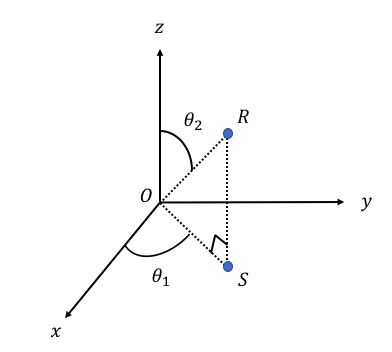
\includegraphics[clip,height= 50mm]{data/theta_sample.png}
\end{center}
\caption{三次元極座標での$\theta_1, \theta_2$の定義}
\label{thetasample}
\end{figure}
\end{frame}

\begin{frame}{混合射影正規分布(1/3)}

$m$個のコンポーネントからなる球面上の混合射影正規分布を以下に示す. 

\vspace{-0.3cm}
\begin{eqnarray*}
\label{MPNS}
p(\bm \theta;\bm w,\bm \mu, \Sigma) = \sum^m_{j=1} w_j \mathcal{PN}_3(\bm \theta;\bm \mu_j, \Sigma_j),
\end{eqnarray*}

\noindent
ただし, $w_j$は混合比率であり, $0 < w_j < 1$, $\sum^m_{j=1} w_j = 1$を満たす. 混合射影正規分布におけるパラメータは, $w, \bm \mu_j, \Sigma_j$であるが, 識別性を考慮して分散共分散行列を定式化する必要がある. 分散共分散行列を以下に示す.
%% 識別性を考慮してとは???
%% どこか1つを1と仮定すれば, そのスケールに合わせて他の変数が移動する的な.

\vspace{-0.3cm}
\begin{eqnarray*}
\label{SIGMA}
 \Sigma_j = \left(
    \begin{array}{cc}
      \Sigma^*_j + \bm \gamma_j \bm \gamma_j^T & \bm \gamma_j \\
      \bm \gamma_j^T & 1
    \end{array}
  \right),
\end{eqnarray*}
\noindent
ここで, $\Sigma^*_j$は$(2 \times 2)$の正定値対称行列, $\bm \gamma_j$は$(2 \times 1)$のベクトルである. パラメータベクトルは$\bm \eta = (w_1, \dots, w_m, \bm \mu_1^T, \dots, \bm \mu_m^T, \mbox{vec}(\Sigma^*_1)^T, \dots, \mbox{vec}(\Sigma^*_m)^T, \bm \gamma_1^T, \dots, \bm \gamma_m^T)^T$となる.

\end{frame}

\begin{frame}{混合射影正規分布(2/3)}
角度データ $\bm \theta$ が得られたときの, パラメータベクトル $\bm \eta$の事後分布を, 事前分布を $p(\bm \eta)$を用いて以下で表せる.

\begin{eqnarray*}
\label{BAYES}
p(\bm \eta | \bm \theta) = \frac{p(\bm \theta | \bm \eta) p(\bm \eta)}{p(\bm \theta)} \propto p(\bm \theta | \bm \eta) p(\bm \eta)
\end{eqnarray*}

\noindent
すなわち, 事後分布$p(\bm \eta | \bm \theta)$は尤度$p(\bm \theta | \bm \eta)$と事前分布 $p(\bm \eta| \bm \theta)$の積に比例する. 尤度と事前分布の計算は簡単であるが, 周辺分布 $p(\bm \theta)$の計算は一般に簡単ではないので, 事後分布に比例する分布 $p(\bm \theta | \bm \eta) p(\bm \eta)$ から乱数サンプルを発生させる. この方法で得られたサンプルをMCMCサンプルと呼ぶ. 
\end{frame}
\begin{frame}{混合射影正規分布(3/3)}

\begin{itemize}
	\item 球面上における混合射影正規分布の尤度関数を以下に示す.
\end{itemize}

\vspace{-0.5cm}
\footnotesize %式を小さくする
\begin{eqnarray*}
\label{logPNS}
\log p(\bm \theta | \bm \eta) + \log p(\bm \eta) &=& \sum^m_{j=1} \{\log w_j + \log \mathcal{PN}_3(\bm \theta;\bm \mu_j, \Sigma_j)\} + \log p(\bm \eta) \\
&\propto& \sum^m_{j=1} \left[ \log w_j - \frac{3}{2} \log A(\bm \theta) - \frac{1}{2} \log |\Sigma_j| + C \right. \\
&&\left. + \log \left( \left[1 + D(\bm \theta) \frac{\Phi \{D(\bm \theta)\}}{\phi \{D(\bm \theta)\}} \right] D(\bm \theta) + \frac{\Phi \{D(\bm \theta)\}}{\phi \{D(\bm \theta)\}} \right) \right] + \log p(\bm \eta), 
\end{eqnarray*}
\normalsize

\noindent
ここで, $D(\bm \theta) = B(\bm \theta) A^{-\frac{1}{2}}(\bm \theta),
A(\bm \theta) = \bm u^T \Sigma^{-1} \bm u,\ B(\bm \theta) = \bm u^T \Sigma^{-1} \bm \mu,$ $\ C = -\frac{1}{2} \bm \mu^T \Sigma^{-1} \bm \mu$である.
\end{frame}

%%%%%%%%%%% 解析手法 %%%%%%%%%%%%%
\section{解析手法}
\begin{frame}{混合分布によるクラスタリング(1/2)}
%\begin{itemize}
\begin{enumerate}
\item
混合分布によるクラスタリングは, 対象となるデータが$m$個のコンポーネントからなる混合データであると仮定し, 混合分布におけるパラメータベクトル$\bm \eta$を推定する. 
\item
得られたパラメータベクトルとデータから, 各データがどのコンポーネントに所属しているかを確率的に表すことができる. 最も高い確率を示す, コンポーネントの番号をデータのラベルとすることで, 各データをクラスタリングすることができる. 
\item
ここでの番号は, 各コンポーネントを表す, 名義尺度なので数値的な意味は存在しない. パラメトリックなクラスタリング手法では, 得られたパラメータベクトル$\bm \eta$の事後分布を用いて, 推定した混合分布の妥当性を検証することができる.	
 
%\end{itemize}
\end{enumerate}

\end{frame}

\begin{frame}{混合分布によるクラスタリング(2/2)}

\begin{itemize}
	\item 混合分布によるクラスタリングでは, $\alpha$は, コンポーネント1に所属し, $\beta$はコンポーネント2に所属しているとする.
\end{itemize}
\begin{figure}[tbp]
\begin{center}
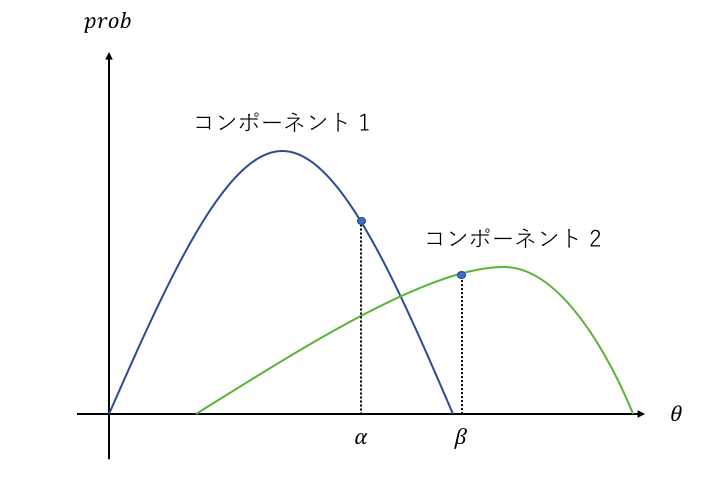
\includegraphics[clip,height= 50mm]{data/mix_cluster.png}
\end{center}
\caption{混合分布によるクラスタリング分析例}
\label{mix_cluster}
\end{figure}


\end{frame}

%%%%%%%%%%% シミュレーション %%%%%%%%%%%%%
\section{シュミレーション}
\begin{frame}{シュミレーション(1/3)}

\begin{itemize}
\item
シミュレーションではコンポーネントを$4$として, $4$つの異なる射影正規分布に従う乱数を混合することで, 混合射影正規分布の人工データを生成する.
\item
サンプリング数を$20000$回, バーンイン期間を$10000$回として, MCMCサンプリングによりパラメータを推定した.

\end{itemize}

\begin{table}[tbp]
\begin{center}
\caption{MCMCによる混合射影正規分布のパラメータ推定}
\label{cross1}
\begin{tabular}{c|c c c c|c c c c}
\hline
  & \multicolumn{4}{c}{真値} & \multicolumn{4}{c}{予測値}\\ \hline
  & 1 & 2 & 3 & 4 & 1 & 2 & 3 & 4 \\ \hline 
$\theta_1$ & 0 & 1.57 & 0.58 & 0.78 & 6.20 & 1.57 & 0.82 & 0.72 \\ 
$\theta_2$ & 1.57 & 0.24 & 1.57 & 0.95 & 1.78 & 0.24 & 1.58 & 1.01\\
$w_j$ & 0.25 & 0.25 & 0.25 & 0.25 & 0.24 & 0.27 & 0.20 & 0.29\\
\hline
\end{tabular}
\end{center}
\end{table}

\end{frame}

\begin{frame}{シュミレーション(2/3)}

\begin{itemize}
	\item 
	横軸を真のコンポーネント, 縦軸を予測のコンポーネントとして集計表を表\ref{cross2}に示す.
\end{itemize}

\begin{table}[tbp]
\begin{center}
\caption{混合射影正規分布によるクラスタリング分析}
\label{cross2}
\begin{tabular}{c|c|c c c c}
\hline
 &  & \multicolumn{4}{c}{予測値} \\ \hline
 &  & 1 & 2 & 3 & 4  \\ \hline 
 & 1 &  \textbf{301} & 27  & 94 & 78 \\ 
真値
 & 2 & 2 & \textbf{473} & 1 & 24 \\
 & 3 & 140 & 14 & \textbf{274} &72 \\ 
 & 4 & 80 & 61 & 44 & \textbf{315} \\ 
\hline
\end{tabular}
\end{center}
\end{table}
\end{frame}

\begin{frame}{シュミレーション(3/3)}

\vspace{-1zh}
\begin{figure}[H]
\begin{tabular}{c}

\begin{minipage}{0.5\hsize}
\begin{center}
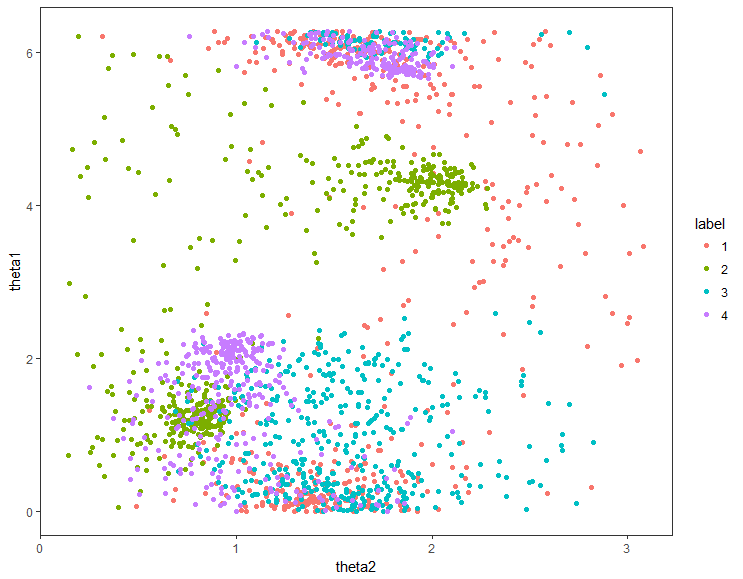
\includegraphics[clip,height= 45mm]{data/real.png}
\end{center}
\end{minipage}

\begin{minipage}{0.5\hsize}
\begin{center}
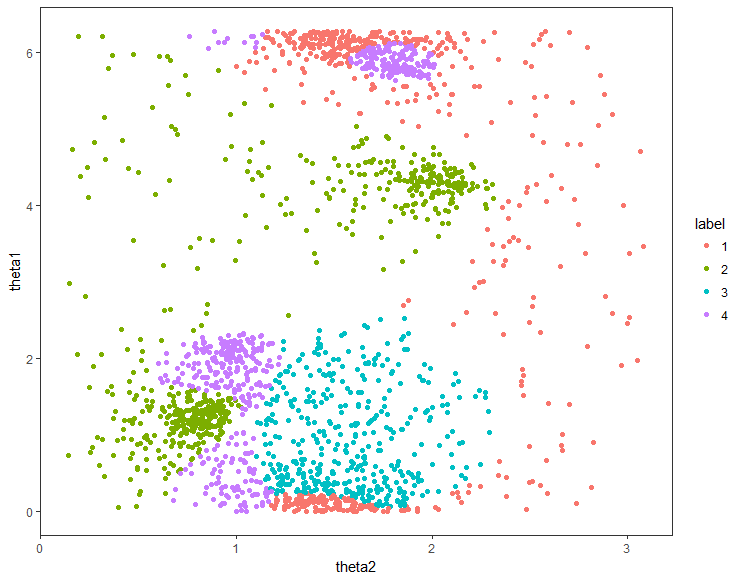
\includegraphics[clip,height= 45mm]{data/pred.png}
\end{center}
\end{minipage}
\end{tabular}
\caption{人工データの角度$\bm \theta = (\theta_1, \theta_2)^T$における散布図(左), 球面上の角度$\bm \theta = (\theta_1, \theta_2)^T$におけるクラスタリング結果(右)}
\end{figure}

\begin{itemize}
\item
各コンポーネントのデータが入り混じっている部分を, クラスタリングにより入り混じることなく分類されていることが分かる. 混合分布によるクラスタリングでは, 複数の分布が密集している部分では, 誤差が大きくなると考えられる.
\end{itemize}

\end{frame}

%%%%%%%%%  データ解析 %%%%%%%%%%%%
\section{データ解析}
\begin{frame}{解析データ(1/2)}

本研究では, GroupLens による公開データセットMovieLensの一部分を用いた. MovieLensデータセットは映画評価サイト''movielens.com''において1997年9月から1998年4月までの7ヶ月間の間に集められた943人のユーザ, 1682個の映画についての評価値が記録されている. 

\begin{table}[bp]
\begin{center}
\caption{コンテンツ情報およびユーザ情報}   %キャプション
\label{MovieLens1}   %ラベル
\scalebox{0.7}{
\begin{tabular}{c l}
\hline
ジャンル & unknown, Action, Adventure, Animation, Children's, Comedy, \\
                 & Crime, Documentary, Drama, Fantasy, Film-Noir, Horror, Musical, \\
                 & Mystery, Romance, Sci-Fi, Thriller, War, Western \\
職業          & administrator, artist, doctor, educator, engineer, entertainment, executive, \\
                & healthcare, homemaker, lawyer, librarian, marketing, none, other, \\
                & programmer, retired, salesman, scientist, student, technician, writer \\
年齢 & 7歳 $\sim$ 73歳 \\
性別 & male, female\\ 
評価値 & 0 $\sim$ 6 (0は見ていない映画への評価) \\
\hline
\end{tabular}
}
\end{center}
\end{table}

\end{frame}

\begin{frame}{解析データ(2/2)}

\begin{enumerate}
	\item 
	943人のユーザの1682個の評価値を, $(943 \times 1682)$ の行列に表現する.
	\item 
	t-SNEを用いて, 行列データの次元を圧縮し, $(943 \times 3)$ の行列とする.
	\item 
	各ユーザのデータを正規化し, 単位球面上にデータを分布させることで, 混合射影正規分布によるクラスタリングを適用する.
\end{enumerate}
\end{frame}


\begin{frame}{コンポーネントの評価指標}

情報量基準(WAIC)を用いて, 混合分布のコンポーネントの選択を行う. WAICは真の分布, 確率モデル, 事前分布がどのような場合でも用いることができる. WAICは以下で定式化される.

\vspace{-0.3cm}
\begin{eqnarray*}
\mbox{WAIC} = T + \frac{V}{n}, 
\end{eqnarray*}

\noindent
ここで, $V = \Sigma^n_{i=1} \{ E_{\bm \eta}[(\log p(\bm \theta_i| \bm \eta))^2] - E_{\bm \eta}[\log p(\bm \theta_i| \bm \eta)]^2 \},T = - \frac{1}{n} \Sigma^n_{i=1} \log E_{\bm \eta}[p(\bm \theta_i| \bm \eta)]$であり, $n$は$\bm \theta$のデータ数である. また$E_{\bm \eta}[\cdot]$は$\bm \eta$の事後分布の下で評価した期待値である.  

\vspace{-0.3cm}
\begin{table}[tbp]
\caption{WAICによるコンポーネントの選択結果}
\label{WAIC2}
\begin{center}
\scalebox{0.60}{
\begin{tabular}{l | c c c c c c c c c c}
\hline
 & 1 & 2 & 3 & 4 & 5 & 6 & 7 & 8 & 9 & 10 \\ \hline 
$m=1$ & -1014.1 & -1237.0 & -1350.6 & -1009.5 & -1308.8 & -1227.8 & -1152.4 & -902.5 & -1322.6 & -1140.2 \\ 
$m=2$ & -1610.9 & -1675.0 & -1760.4 & -1552.8 & -1633.1 & -1529.6 & -1507.1 & -1366.1 & -1645.2 & -1693.3 \\ 
$m=3$ & -1846.8 & -1744.7 & -1728.9 & -1804.9 & -1741.0 & -1654.3 & -1705.2 & -1633.8 & -1789.3 & \textbf{-1872.1} \\ 
$m=4$ & \textbf{-1893.6} & \textbf{-1969.8} & \textbf{-1901.6} & \textbf{-1837.5} & \textbf{-1787.5} & \textbf{-1687.8} &\textbf{-1749.5} & \textbf{-1686.7} & \textbf{-1844.5} & -1802.6 \\ 
\hline
\end{tabular}
}
\end{center}
\end{table}

\end{frame}

\begin{frame}{データ解析(1/3)}

\begin{itemize}
	\item 
	コンポーネントを$4$つと仮定して混合射影正規分布によるクラスタリングを行う. サンプリング数を$20000$回, バーンイン期間を$10000$回として, MCMCサンプリングによりパラメータを推定した.
	\item
	$4$つのコンポーネントにおける混合射影正規分布のパラメータを以下に示す. なお, $\hat {\bm w}$は各コンポーネントの混合比率を表し, パラメータの添え字は各コンポーネントの番号に対応している.
\end{itemize}
 
\footnotesize %式を小さくする
\begin{equation*}
\begin{split}
&\hat {\bm w} = \begin{pmatrix} 0.26 \\ 0.51 \\ 0.20 \\ 0.03 \\ \end{pmatrix},\ 
\hat{\bm \mu}_1 = \begin{pmatrix} 0.44 \\ 2.85 \\ -1.67 \\ \end{pmatrix},\ 
\hat \Sigma_1 = \begin{pmatrix}  2.40 & 1.52 &  0.06 \\ 1.52 & 2.20 & -0.25 \\ 0.06 & -0.25 &1.00 \\ \end{pmatrix},\\ 
&\hat{\bm \mu}_2 = \begin{pmatrix} 0.14 \\ -0.50 \\ 1.09 \\ \end{pmatrix},\ 
\hat \Sigma_2 = \begin{pmatrix}   0.28  & 0.14 &  0.20 \\ 0.14 & 0.61 & 0.06 \\  0.20 & 0.06 &1.00 \\ \end{pmatrix},\ 
\hat{\bm \mu}_3 = \begin{pmatrix} -2.08  \\ -1.96 \\ -8.11 \\ \end{pmatrix},\\ 
&\hat \Sigma_3 = \begin{pmatrix}  1.86  & -0.18 &  -0.10 \\-0.18 & 3.89 & 1.60 \\  -0.10 & 1.60 & 1.00 \\ \end{pmatrix},\ 
\hat{\bm \mu}_4 = \begin{pmatrix} -12.29   \\ -2.48 \\ -4.84 \\ \end{pmatrix},\ 
\hat \Sigma_4 = \begin{pmatrix} 15.19 & 4.01 &  0.12 \\ 4.01 & 1.88 & 0.08 \\ 0.12 & 0.08 &1.00 \\ \end{pmatrix}.
\end{split}
\end{equation*}
\normalsize
\end{frame}


\begin{frame}{データ解析(2/3)}

\vspace{-1zh}
\begin{figure}[H]
\begin{tabular}{c}

\begin{minipage}{0.5\hsize}
\begin{center}
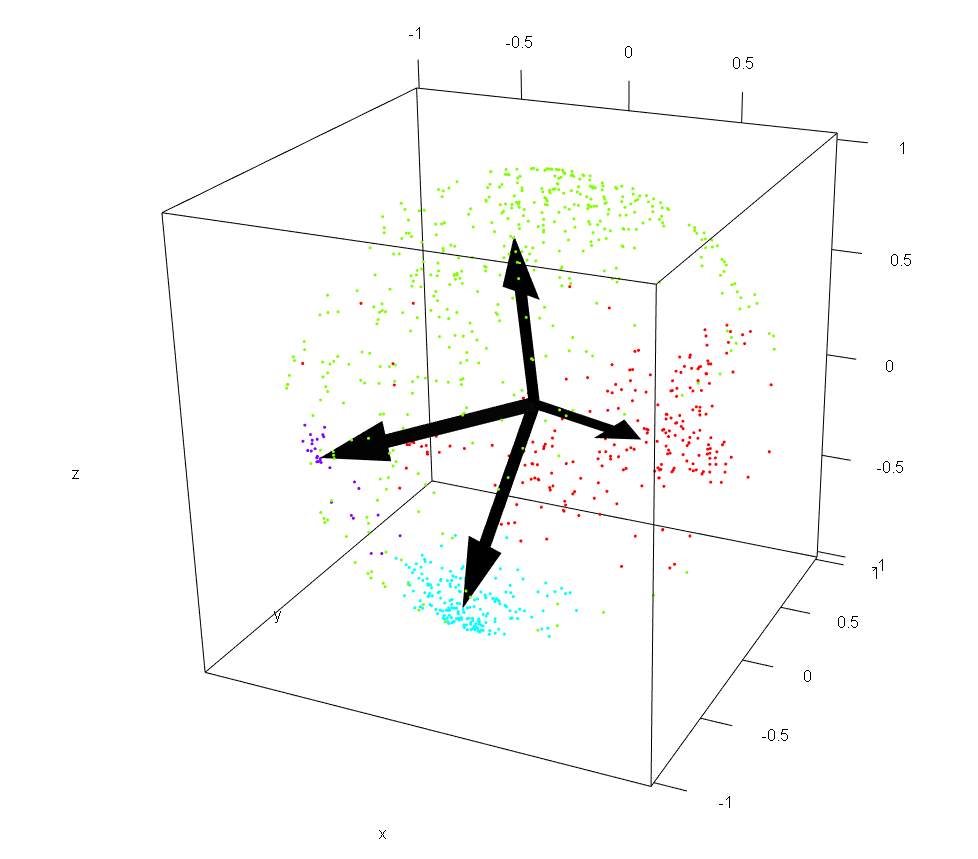
\includegraphics[clip,height= 40mm]{data/cluster_3d.png}
\end{center}
\end{minipage}

\begin{minipage}{0.5\hsize}
\begin{center}
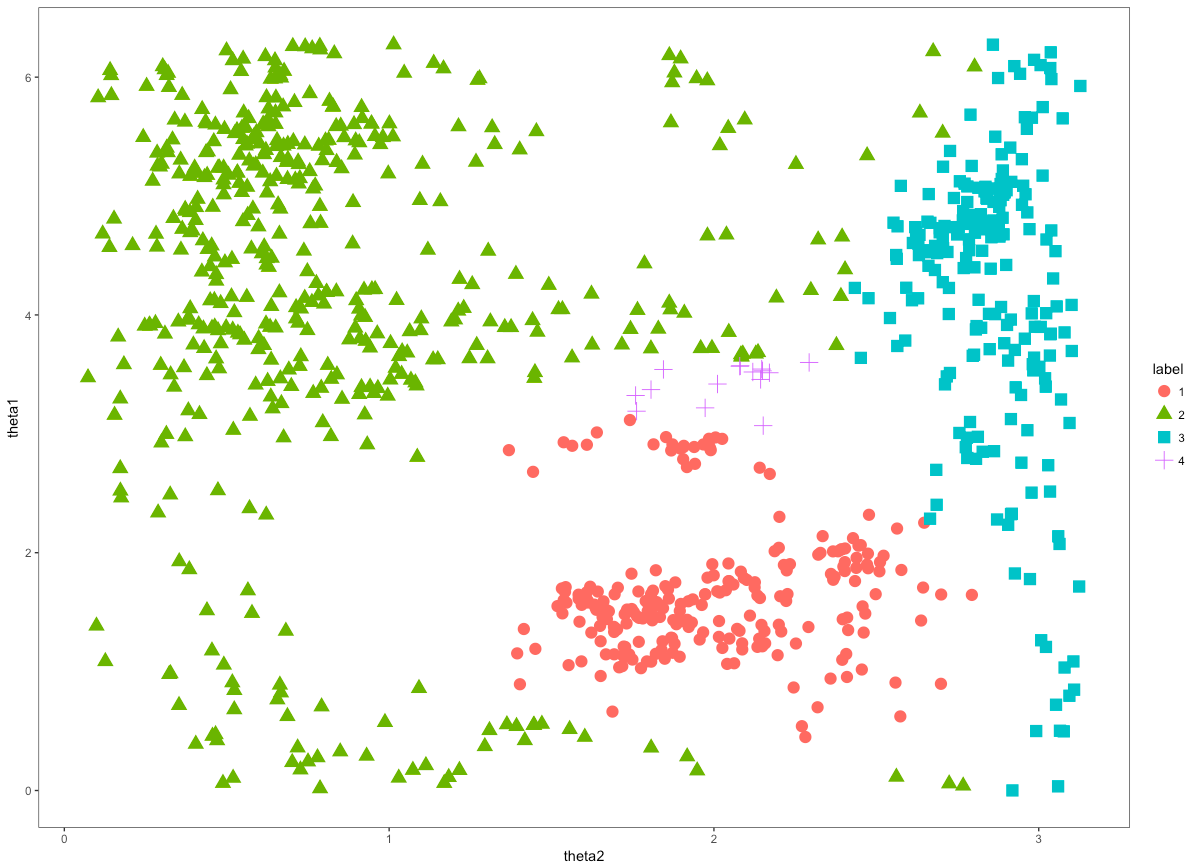
\includegraphics[clip,height= 40mm]{data/cluster_4.png}
\end{center}
\end{minipage}

\end{tabular}
\label{fig2}
\caption{混合分布による, 球面上におけるクラスタリング結果(左), 混合分布による, 球面上の角度$\bm \theta = (\theta_1, \theta_2)^T$におけるクラスタリング結果(右)}
\end{figure}
\end{frame}

\begin{frame}{データ解析(3/3)}
\begin{figure}[tbp]
\begin{center}
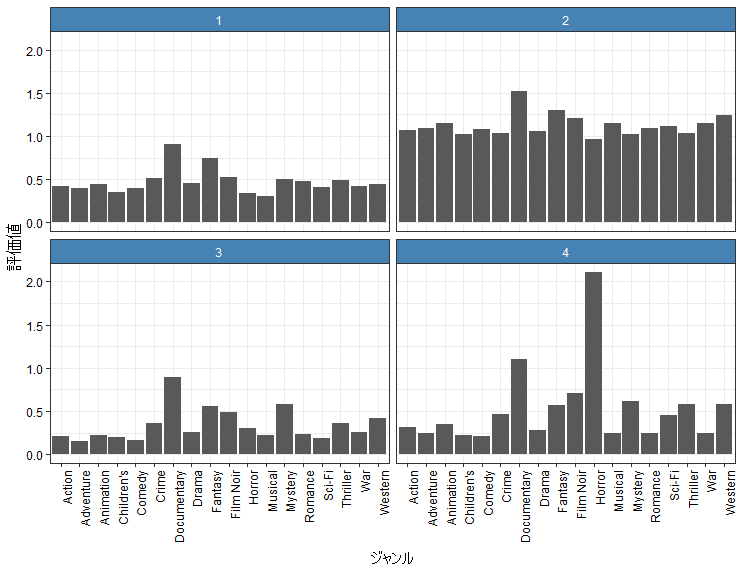
\includegraphics[clip,height= 55mm]{data/cluster_plot.png}
\end{center}
\caption{クラスターごとのジャンルへの評価値}
\label{clustergenre}
\end{figure}

\begin{itemize}
	\item コンポーネント2はすべてのジャンルへの評価値が高く, その他のコンポーネントでは, ジャンルへの評価値に差異が現れた.
\end{itemize}
\end{frame}

%%%%%%%%%%%%%% まとめと今後の課題 %%%%%%%%%%%%%%%%%
\section{まとめと今後の課題}
\begin{frame}{まとめと今後の課題}

\begin{itemize}

\item
一般化射影正規分布では任意次元の超球面において分布を生成することができるので, 計算量の問題を解決し, 次元を圧縮することなく超球面上でのクラスタリングに取り組みたい. 
\item
数値データを球面上に配置し, クラスタリングを行ったのが, 超球面上でのクラスタリングは主にテキストマイニングや画像データに用いられているので, それらのデータに対するパラメトリックなクラスタリングを行い, 従来手法との比較を行いたい. 

\end{itemize}

\end{frame}

\section{参考文献}
\begin{frame}{参考文献}

{\scriptsize
\begin{thebibliography}{99}
%\setlength{\itemsep}{-.5zw}
\beamertemplatetextbibitems %参考文献に番号を振る

\bibitem{GPN}
D.Hernandez-Stumpfhauser and F. J. Breidt and Mark J. van der Woerd. (2017). The General Projected Normal Distribution of Arbitrary Dimension: Modeling and Bayesian Inference. {\it Journal of Bayesian Analysis}, Vol. 12, No. 1, pp. 113-133.

\bibitem{PN1}
F. Wang and A. E. Gelfand. (2013). Directional data analysis under the general
projected normal distribution. {\it Statistical Methodology}, Vol.10, pp. 113-127.

\bibitem{PN2}
B. Presnell, S. P. Morrison, and R. C. Littell. (1998). Projected multivariate linear models for
directional data. {\it Journal of the American Statistical Association}, Vol. 443, pp. 1068-1077.

%\bibitem{mvonMF}
%Jalil Taghia and Zhanyu Ma and Arne Leijon. (2014). Bayesian Estimation of the von-Mises Fisher Mixture %Model with Variational Inference. {\it IEEE}, Vol.36, No. 9, pp. 1701-1715.

\bibitem{vonMF}
S. Gopal and Y. Yang. (2014). Von Mises-Fisher Clustering Models. {\it ICML}.

\bibitem{skmeans}
S. Dhillon and S. Modha. (2001). Concept Decompositions for Large Sparse Text Data Using
Clustering. {\it Machine Learning}, Vol. 42, pp. 143-175.

\bibitem{movie}
GroupLensホームページ(http://movielens.org/.) 

\end{thebibliography}
}

\end{frame}

%%%%%%%%%%%%%%付録%%%%%%%%%%%%%%%%付録%%%%%%%%%%%%%%
\backupbegin
\begin{frame}{識別性}
\begin{itemize}
	\item 
	識別性とは, 異なるパラメータにおいて, $p(\theta; \mu_1, \Sigma_1)$と$p(\theta; \mu_2, \Sigma_2)$が異なるということである. 射影正規分布は異なるパラメータでも同様の確率分布をとることがあるため, 分散パラメータの$1$つを固定して, 識別性を保持する.
\end{itemize}

\begin{figure}[htbp]
 \begin{tabular}{c}
 %\hspace{0.5cm}
 \begin{minipage}{0.5\hsize}
  \begin{center}
   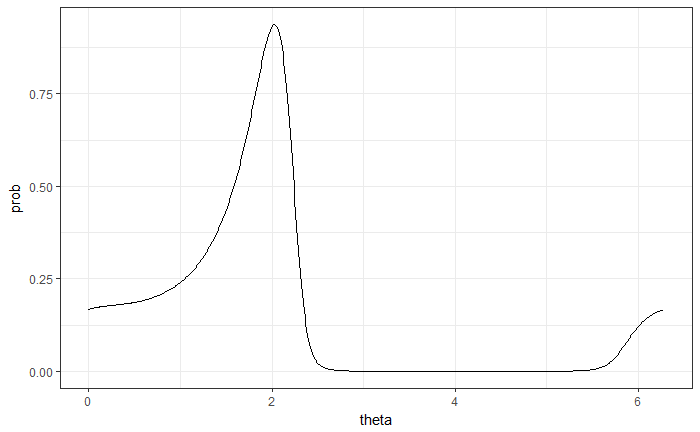
\includegraphics[clip,height= 30mm]{data/pn_sikibetu_real.png}
  \end{center}
 \end{minipage}
 \begin{minipage}{0.5\hsize}
  \begin{center}
 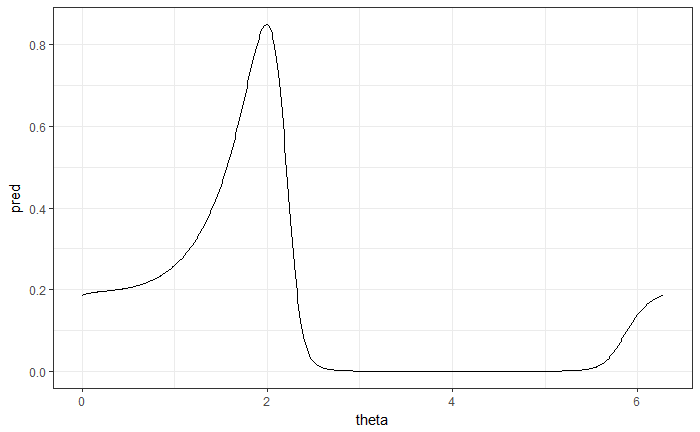
\includegraphics[clip,height= 30mm]{data/pn_sikibetu_pred.png}
  \end{center}
 \end{minipage}
\end{tabular}
\caption{異なるパラメータにおける射影正規分布の分布例}
\end{figure}

\end{frame}

\begin{frame}{t-SNE(1/2)}

t-SNEは高次元データの次元を圧縮するアルゴリズムであり, 特に高次元データを可視化する際に有用である. このアルゴリズムでは高次元空間における$2$点間の近さを確率分布として表現する. 高次元データ$\bm x$を低次元データ$\bm y$に近似するとき, 次元圧縮前の点$x_j$と点$x_i$の類似度を条件付確率$P_{j|i}$を用いて, 同時確率$P_{ij}$で表し, 次元圧縮後の点$y_j$と点$y_i$の類似度を同時確率$Q_{ij}$によって表す.

\footnotesize
\begin{eqnarray*}
\label{tsne1}
P_{j|i} = \frac{\exp(-\|x_i - x_j\|^2 / 2\sigma_i^2}{\Sigma_{k \neq i}\exp(-\|x_i - x_k\|^2/ 2\sigma_i^2)},\ 
P_{ij} = \frac{P_{j|i} + P_{i|j}}{2N},\ 
Q_{ij} = \frac{(1 + \|y_i - y_j\|^2)^{-1}}{\Sigma_{k \neq i}(1 + \|y_i - y_k\|^2)^{-1}},
\end{eqnarray*}
\normalsize

\noindent
ここで, $\sigma_i$は点$x_i$を中心とした正規分布における, 任意の分散パラメータである.
\end{frame}

\begin{frame}{t-SNE(2/2)}

圧縮前の確率分布と圧縮後の確率分布のKL情報量を損失関数$L$として, $L$が最小になるような$y_i$を求めることで, 低次元データ$\bm y$を取得する. 損失関数$L$を以下に示す.

\begin{eqnarray*}
\label{tsne3}
L = KL(P || Q) = \Sigma_i \Sigma_j P_{ij} \log \frac{P_{ij}}{Q_{ij}}.
\end{eqnarray*}
\end{frame}

\begin{frame}{HMC(1/2)}

MCMCアルゴリズムの一つである, ハミルトニアン$\cdot$モンテカルロ法(HMC)を用いて分布の推定を行う. ハミルトニアンとはポテンシャルエネルギー $U(\bm \eta)$ と運動エネルギー $V(\bm q)$ の和で定義される物理量 $H(\bm \eta, \bm q) = U(\bm \eta) + V(\bm q)$ のことであり. ここで, $\bm q = (q_1, \dots, q_d)^T$ は$\bm \eta$ と同じ$d$次元のベクトルである. $t$番目のステップにおける, ハミルトニアン方程式は以下で定義される. 

\begin{eqnarray*}
\label{HMC}
\frac{d \eta_j(t)}{dt} = \frac{\partial V(\bm q)}{\partial q_j},\ \ \frac{d q_j(t)}{dt} = - \frac{\partial U(\bm \eta)}{\partial \eta_j},
\end{eqnarray*}
\end{frame}

\begin{frame}{HMC(2/2)}

\begin{enumerate}

\item{}
$\eta_j(0), q_j(0)$の初期値を設定する. $\eta_j(0)$は各パラメータの事前分布からの設定し, $q_j(0)$は$N(0,M_j)$からランダムサンプリングする. $M_j$ は任意の分散パラメータである. 
 
\item{}

以下の式に従い, $\eta_j, \bm q_j$を更新する. $\epsilon$は状態変化のステップ幅を表す.
\footnotesize
\begin{eqnarray*}
&&q_j(t+\frac{\epsilon}{2}) = q_j(t) - \frac{\epsilon}{2} \frac{\partial U}{\partial \eta_j} (\bm \eta(t)),\ 
\eta_j(t+\epsilon) = \eta_j(t) + \epsilon \frac{q_j(t + \frac{\epsilon}{2})}{M_j},\\ 
&&q_j(t+\epsilon) = q_j(t+\frac{\epsilon}{2}) - \frac{\epsilon}{2} \frac{\partial U}{\partial \eta_j} (\bm \eta(t + \epsilon)),
\end{eqnarray*}
\normalsize

\item{}
得られたパラメータの採択, 棄却を決定する. 上記のステップで得られたパラメータを$\eta^*_j, q^*_j$として,
現在が$t$回目の反復とすると, サンプルの棄却率は以下の式で定義する.

\vspace{-0.5cm}
\begin{eqnarray*}
r_j = \frac{p(\eta^*_j|\theta_j) p(q^*_j)}{p(\eta_j(t-1)|\theta_j) p(q_j(t-1))}.
\end{eqnarray*}

\item{}
一様乱数 $u_j \sim U(0,1)$を発生し, $r_j > u_j$ならば, ランダムサンプル $\eta^*_j$を採択し, $r_j < u_j$ならば, $\eta_j(t-1)$を保持する. サンプル数$T$が任意の数に達したとき, MCMCサンプリングを終了する. 

\end{enumerate}

\end{frame}

\begin{frame}{ジャンルへの評価値の算出方法(1/2)}
各ユーザの評価値と各映画のジャンル($19$種類)を用いて, ユーザごとに各ジャンルへの総評価値を算出する. 各映画には複数のジャンルが対応している. ユーザごとに全ての映画に対して, 

\begin{equation*}
\mbox{(任意の映画に対する評価値)} \times \mbox{(任意の映画のジャンル)},
\end{equation*}

\noindent
を算出し, 総和をとることで, ユーザごとに各ジャンルへの総評価値を求めた. これらの計算は, ユーザー($943$人)$\times$コンテンツ($1682$個)の行列とコンテンツ($1682$個)$\times$ジャンル($19$個)の行列の演算に相当しており, 省略形を以下に示す. 

\footnotesize %式を小さくする
\begin{equation*}
\label{user_genre_matrix}
\begin{pmatrix} 
5 & 3 & 4 & 3 & \ldots & 0 \\
4 & 0 & 0 & 0 & \ldots & 0 \\
\vdots & \vdots & \vdots & \vdots & \ddots & \vdots \\
0 & 5 & 0 & 0 & \ldots & 0 \\
\end{pmatrix} 
\times
\begin{pmatrix} 
0 & 0 & \ldots & 0 \\
0 & 1 & \ldots & 0 \\
0 & 0 & \ldots & 0 \\
0 & 1 & \ldots & 0 \\
\vdots & \vdots & \ddots & \vdots \\
0 & 0 & \ldots & 0 \\
\end{pmatrix}
=
\begin{pmatrix} 
0 & 95 & \ldots & 4 \\
0 & 17 & \ldots & 0 \\
0 & 17 & \ldots & 0 \\
\vdots & \vdots & \ddots & \vdots \\
0 & 227 & \ldots & 23 \\
\end{pmatrix},
\end{equation*}
\normalsize

\end{frame}

\begin{frame}{ジャンルへの評価値の算出方法(2/2)}
\noindent
ここで, 得られたユーザごとジャンルへの評価値から, コンポーネントごとのジャンルへの評価値を求める. 図\ref{genre_count}に示すように, 各ジャンルは均等に出現していないので, 各ジャンルの影響を基準化する.

\vspace{0.5cm}
\begin{figure}[htbp]
\begin{center}
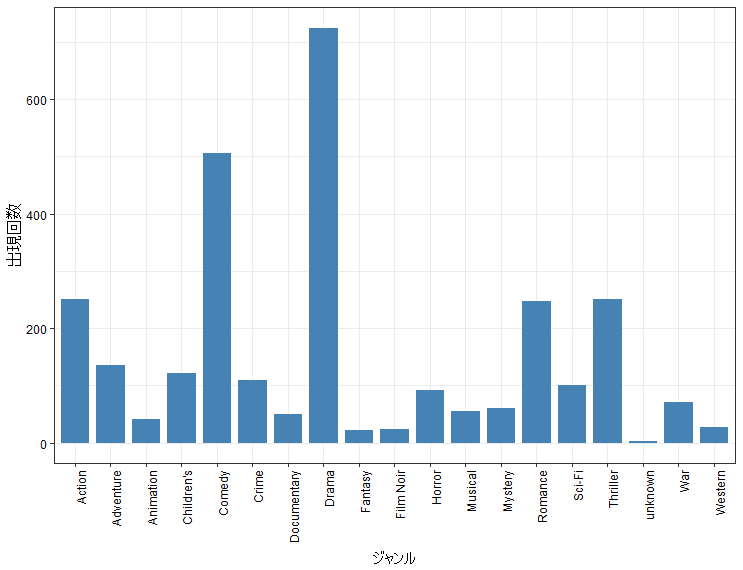
\includegraphics[clip,height= 45mm]{data/genre_count.png}
\end{center}
\caption{コンテンツの各ジャンルの出現回数}
\label{genre_count}
\end{figure}
\end{frame}
	
\backupend
\end{document}

%\vspace{-0.5cm}
%\begin{figure}[H]
% \begin{center}
 % 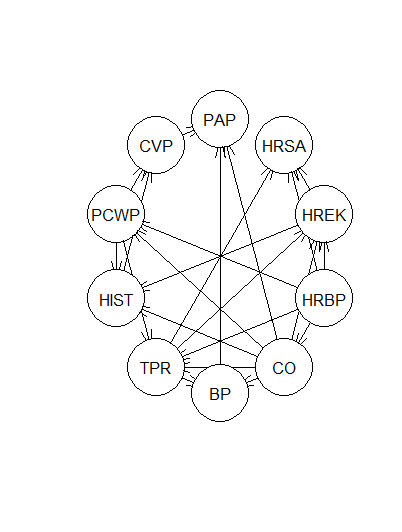
\includegraphics[width=40mm]{data/BN4.png}
 %\end{center}
 %\caption{ベイジアンネットワークの例}
 %\label{naive}
%\end{figure}